\documentclass[border=15pt]{standalone}
\usepackage{tikz,amsmath,amssymb}
\usetikzlibrary{arrows.meta}
\usepackage{tikzcats}   % 原生保留 tikzcats

% ========== 配色方案 ==========
% 编码器（上行：冷暖渐进）
\definecolor{inFill}{RGB}{183,224,177}       % 浅绿 (H/2)
\definecolor{inLine}{RGB}{32,102,32}
\definecolor{blFill}{RGB}{190,225,245}       % 天蓝 (H/4)
\definecolor{blLine}{RGB}{40,110,170}
\definecolor{orFill}{RGB}{250,224,180}       % 橙黄 (H/8)
\definecolor{orLine}{RGB}{190,110,20}
\definecolor{yeFill}{RGB}{252,240,180}       % 鹅黄 (H/16, 骨干深层)
\definecolor{yeLine}{RGB}{180,150,20}

% 解码器（下行：差异化高雅配色，通道全为 K）
\definecolor{decFiveFill}{RGB}{220,210,245}  % 淡紫蓝 (H/16)
\definecolor{decFiveLine}{RGB}{95,70,165}
\definecolor{decFourFill}{RGB}{235,215,245}  % 淡紫 (H/8)
\definecolor{decFourLine}{RGB}{125,55,160}
\definecolor{decThreeFill}{RGB}{248,215,225} % 玫瑰红/藕粉 (H/4)
\definecolor{decThreeLine}{RGB}{180,50,90}
\definecolor{decTwoFill}{RGB}{210,240,235}   % 薄荷青 (H/2)
\definecolor{decTwoLine}{RGB}{25,130,120}

\definecolor{maskBg}{RGB}{35,40,52}         % 分割图深色背景
\definecolor{maskCat}{RGB}{230,60,50}       % 分割猫咪目标红色

% 与 \cat 几何同构的语义分割掩码宏
\def\catmask#1{
\scope[scale=3]
    \draw[line width=15pt, #1, cap=round] (0,-2.3) .. controls +(-2,0) and (-2,-1.3) .. (-1.5,-1);
    \draw[line width=15pt, #1, cap=round] (-1.5,-1) .. controls +(0.9,0.4) and (-1.1,0.1) .. (-1.5,0);
    \fill[#1] (0.5,-2) circle (0.5);
    \fill[#1] (-0.5,-2) circle (0.5);
    \fill[#1, rounded corners=50pt] (-0.5,-2.5) rectangle (0.5,-0.3);
    \fill[#1] (0.4,-2.5) .. controls (0.3,-0.5) and (-0.3,-0.5) .. (-0.4,-2.5);
    \fill[#1] (0.4,-1.6) ellipse (0.2 and 0.9);
    \fill[#1, rounded corners=10pt] (0.6,-2.52) rectangle (0.2,-2.25);
    \fill[#1] (-0.4,-1.6) ellipse (0.2 and 0.9);
    \fill[#1, rounded corners=10pt] (-0.6,-2.52) rectangle (-0.2,-2.25);
    \fill[#1] (0,0) circle (0.65);
    \fill[rounded corners=8pt, #1] (0,0.5) -- (-0.6,1) -- (-0.7,0.8) -- (-0.6,0) -- cycle;
    \fill[rounded corners=8pt, #1] (0,0.5) -- (0.6,1) -- (0.7,0.8) -- (0.6,0) -- cycle;
    \fill[#1] (0,-0.5) ellipse (0.25 and 0.2);
    \draw[line width=1.5pt, #1, cap=round] (0.15,-0.34) .. controls (0.3,-0.31) and (0.6,-0.32) .. (0.8,-0.39);
    \draw[line width=1.5pt, #1, cap=round] (0.15,-0.39) .. controls (0.3,-0.36) and (0.55,-0.42) .. (0.75,-0.49);
    \draw[line width=1.5pt, #1, cap=round] (-0.15,-0.34) .. controls (-0.3,-0.31) and (-0.6,-0.32) .. (-0.8,-0.39);
    \draw[line width=1.5pt, #1, cap=round] (-0.15,-0.39) .. controls (-0.3,-0.36) and (-0.55,-0.42) .. (-0.75,-0.49);
\endscope
}

\begin{document}
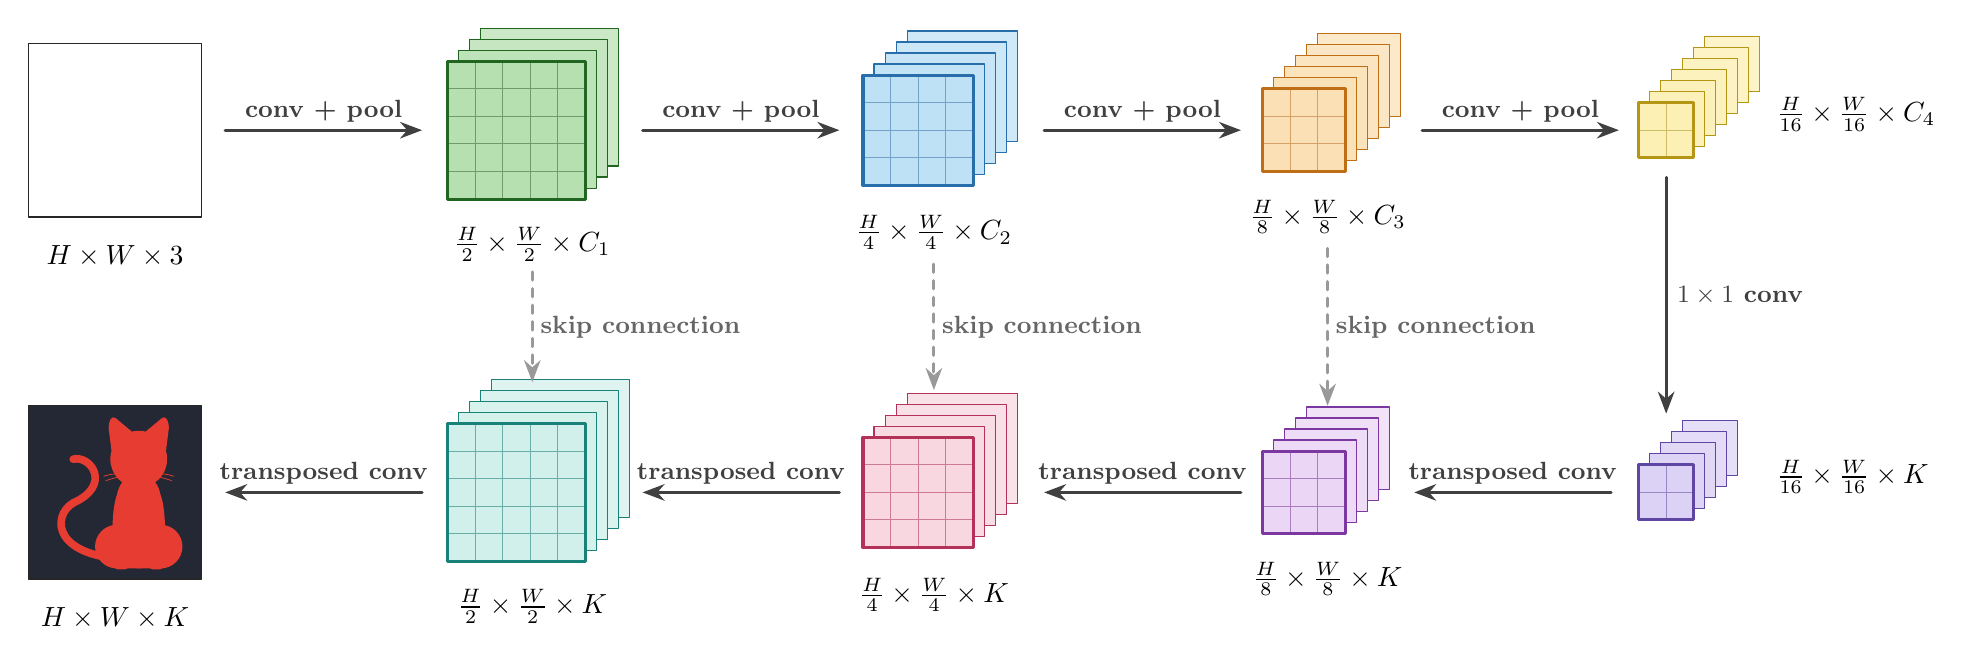
\begin{tikzpicture}[
    font=\normalsize, line join=round, line cap=round,
    every node/.style={inner sep=0pt, outer sep=0pt, align=center},
    arr/.style={->, >=Stealth, line width=1.1pt, darkgray},
    skip/.style={->, >=Stealth, dashed, line width=1.1pt, gray!80}
  ]

  % ========== 宏：优化后的 3D 堆叠特征图 ==========
  \newcommand{\fstack}[6]{%
    \pgfmathsetmacro{\sz}{#4*#5}
    \pgfmathsetmacro{\half}{\sz/2}
    \foreach \k in {#3,...,1}{%
      \pgfmathtruncatemacro{\op}{round(100 - (28 * \k / #3))}
      \fill[#6Fill!\op, draw=#6Line, line width=.4pt]
        ({#1 - \half + 0.14*\k}, {#2 - \half + 0.14*\k}) rectangle ++({\sz}, {\sz});
    }
    \fill[#6Fill] ({#1 - \half}, {#2 - \half}) rectangle ++({\sz}, {\sz});
    \draw[step=#5, #6Line!65, line width=.35pt, shift={({#1 - \half}, {#2 - \half})}] (0,0) grid ({\sz}, {\sz});
    \draw[#6Line, line width=1.1pt] ({#1 - \half}, {#2 - \half}) rectangle ++({\sz}, {\sz});
  }

  % 输入猫咪图片 (2.2 x 2.2 cm)
  \newcommand{\catimg}[2]{%
    \draw[black!85, line width=.5pt, fill=white] ({#1-1.1},{#2-1.1}) rectangle ++(2.2,2.2);
    \node at (#1, #2) {\scalebox{0.185}{\tikz{\cat}}};
  }

  % 语义分割掩码输出图片 (2.2 x 2.2 cm)
  \newcommand{\catmaskimg}[2]{%
    \fill[maskBg] ({#1-1.1},{#2-1.1}) rectangle ++(2.2,2.2);
    \node at (#1, #2) {\scalebox{0.185}{\tikz{\catmask{maskCat}}}};
    \draw[black!85, line width=.5pt] ({#1-1.1},{#2-1.1}) rectangle ++(2.2,2.2);
  }

  % 【上半部分】：下采样编码阶段 (向右流动)
  % 1. Input Image
  \catimg{1.1}{2.6}
  \node[font=\normalsize, text=black] at (1.1, 1.0) {$H\times W\times 3$};

  % 2. 阶段 1: H/2
  \draw[arr] (2.5, 2.6) -- (5.0, 2.6) node[midway, above=3pt, font={\small\bfseries}] {conv + pool};
  \fstack{6.2}{2.6}{3}{5}{0.35}{in}
  \node[font=\normalsize, text=black, fill=white, inner sep=2pt] at (6.4, 1.15) {$\frac{H}{2}\times\frac{W}{2}\times C_1$};

  % 3. 阶段 2: H/4
  \draw[arr] (7.8, 2.6) -- (10.3, 2.6) node[midway, above=3pt, font={\small\bfseries}] {conv + pool};
  \fstack{11.3}{2.6}{4}{4}{0.35}{bl}
  \node[font=\normalsize, text=black, fill=white, inner sep=2pt] at (11.5, 1.3) {$\frac{H}{4}\times\frac{W}{4}\times C_2$};

  % 4. 阶段 3: H/8
  \draw[arr] (12.9, 2.6) -- (15.4, 2.6) node[midway, above=3pt, font={\small\bfseries}] {conv + pool};
  \fstack{16.2}{2.6}{5}{3}{0.35}{or}
  \node[font=\normalsize, text=black, fill=white, inner sep=2pt] at (16.5, 1.5) {$\frac{H}{8}\times\frac{W}{8}\times C_3$};

  % 5. 阶段 4: H/16 (与上行对齐)
  \draw[arr] (17.7, 2.6) -- (20.2, 2.6) node[midway, above=3pt, font={\small\bfseries}] {conv + pool};
  \fstack{20.8}{2.6}{6}{2}{0.35}{ye}
  \node[font=\normalsize, text=black, anchor=west] at (22.2, 2.8) {$\frac{H}{16}\times\frac{W}{16}\times C_4$};

  % 【右侧下行连接】：从上行 H/16 垂直向下到 下行 H/16 (1x1 conv，通道变为 K)
  \draw[arr] (20.8, 2.0) -- (20.8, -1.0) node[midway, right=4pt, font={\small\bfseries}] {$1\times 1$ conv};

  % 【下半部分】：上采样解码阶段 (向左流动，四路转置卷积完全对称)
  % 解码阶段 0: 下行 H/16 (通道数改为 K)
  \fstack{20.8}{-2.0}{4}{2}{0.35}{decFive}
  \node[font=\normalsize, text=black, anchor=west] at (22.2, -1.8) {$\frac{H}{16}\times\frac{W}{16}\times K$};

  % 解码阶段 1: 第 1 个转置卷积 (H/16 -> H/8)
  \draw[arr] (20.1, -2.0) -- (17.6, -2.0) node[midway, above=3pt, font={\small\bfseries}] {transposed conv};
  \fstack{16.2}{-2.0}{4}{3}{0.35}{decFour}
  \node[font=\normalsize, text=black] at (16.5, -3.1) {$\frac{H}{8}\times\frac{W}{8}\times K$};

  % 解码阶段 2: 第 2 个转置卷积 (H/8 -> H/4)
  \draw[arr] (15.4, -2.0) -- (12.9, -2.0) node[midway, above=3pt, font={\small\bfseries}] {transposed conv};
  \fstack{11.3}{-2.0}{4}{4}{0.35}{decThree}
  \node[font=\normalsize, text=black] at (11.5, -3.3) {$\frac{H}{4}\times\frac{W}{4}\times K$};

  % 解码阶段 3: 第 3 个转置卷积 (H/4 -> H/2)
  \draw[arr] (10.3, -2.0) -- (7.8, -2.0) node[midway, above=3pt, font={\small\bfseries}] {transposed conv};
  \fstack{6.2}{-2.0}{4}{5}{0.35}{decTwo}
  \node[font=\normalsize, text=black] at (6.4, -3.45) {$\frac{H}{2}\times\frac{W}{2}\times K$};

  % 解码阶段 4: 第 4 个转置卷积 (H/2 -> HxW 全尺寸输出)
  \draw[arr] (5.0, -2.0) -- (2.5, -2.0) node[midway, above=3pt, font={\small\bfseries}] {transposed conv};
  \catmaskimg{1.1}{-2.0}
  \node[font=\normalsize, text=black] at (1.1, -3.6) {$H\times W\times K$};

  % 【跳跃连接】：灰色虚线垂直下连 (Skip Connections)
  % 1. H/8: 顶部 H/8 垂直连接到底部 H/8
  \draw[skip] (16.5, 1.1) -- (16.5, -0.9)
    node[pos=0.5, right=3pt, font={\small\bfseries}, text=gray!80!black] {skip connection};

  % 2. H/4: 顶部 H/4 垂直连接到底部 H/4
  \draw[skip] (11.5, 0.9) -- (11.5, -0.7)
    node[pos=0.5, right=3pt, font={\small\bfseries}, text=gray!80!black] {skip connection};

  % 3. H/2: 顶部 H/2 垂直连接到底部 H/2
  \draw[skip] (6.4, 0.8) -- (6.4, -0.6)
    node[pos=0.5, right=3pt, font={\small\bfseries}, text=gray!80!black] {skip connection};

\end{tikzpicture}
\end{document}